\chapter{Измерение информации Вигнера-Янасе в МК эксперименте ЯМР}
\label{chapter:wyi-mesuarement}

% PLA-2021

В разделе~\ref{sec:manyparticle-entanglement-criteria} был обсужден критерий многочастичной запутанности
в терминах обобщенной информации.
В свою очередь в разделах~\ref{sec:quantum-fisher-information}~и~\ref{sec:skew-wigner-yanase-information}
было показано,
что в качестве такой обобщённой меры информации могут выступать
квантовая информация Фишера и косая информация Вигнера-Янасе.
Тем не менее в предыдущих разделах многочастичная запутанность была исследована исключительно
на основе квантовой информации Фишера.
Главной причиной такого выбора является тот факт,
что нижняя граница квантовой информации Фишера может быть измерена в МК эксперимента ЯМР~(см.  раздел~\ref{sec:quantum-fisher-information-mesuarement-at-high-temperature}),
и, следовательно, многочастичная запутанность может быть исследована экспериментально.
В этой главе будет продемонстрировано,
что и косая информация Вигнера-Янасе связана с
со вторым моментом МК спектра ЯМР,
а также проведено сравнение оценок многоспиновой запутанности
на основе косой информации Вигнера-Янаса и квантовой информации Фишера.



\section{Связь косой информации и второго момента МК спектра ЯМР}
\label{sec:wyi-mesuarement}

Для прояснения связи косой информации Вигнера-Янаса и
второго момента интенсивностей МК когерентностей ЯМР,
ниже будет получено выражение для косой информации
на подготовительном периоде МК эксперимента ЯМР~(см. раздел~\ref{sec:mq-nrm-experiment})
с начальным термодинамически равновесным состоянием $\rho_\mathrm{eq}$.
Матрица плотности системы в начальный момент времени имеет вид:
\begin{equation}
  \rho(0, \beta)
  = \rho_\mathrm{eq}
  = \dfrac{e^{\frac{\hbar\omega_{0}}{kT} I_z}}{Z}
  = \dfrac{e^{\beta I_z}}{Z},
\end{equation}
где $Z = \tr{e^{\beta I_z}}$ --- статистическая сумма,
$\hslash$ и $k$ --- константы Планка и Больцмана,
$\omega_{0}$ --- частота Лармора,
$I_\mathrm{z}$ ---  оператор проекции полного углового спинового момента  на ось~$z$,
который направлен вдоль сильного внешнего магнитного поля.
Эволюционная матрица плотности $\rho(\tau,\beta)$ на подготовительном периоде
под действием стационарного гамильтониана $H_\mathrm{MQ}$
может быть получена из уравнения Лиувилля,
которое имеет вид
%
\begin{equation}\label{eq:rho-eval}
  \rho(\tau,\beta)
  = V^+(\tau) \rho(0, \beta) V(\tau)
  = V^+(\tau) \frac{e^{\beta I_z}}{Z} V(\tau),
\end{equation}
где $V(\tau) = e^{iH_\mathrm{MQ}\tau}$
--- это оператор эволюции.

Косая информация Вигнера-Янасе определяется выражением~(см. раздел~\ref{sec:skew-wigner-yanase-information})
%
\begin{equation}\label{eq:wyi}
  I_{WY}(\rho(\tau,\beta),I_z)
  = -\frac{1}{2} Tr([\sqrt{\rho(\tau,\beta)},\sigma_z])^2
  = -2 Tr([\sqrt{\rho(\tau,\beta)},I_z])^2,
\end{equation}
%
где $\sigma_z=2I_z$ --- это оператор Паули.
Интригующей особенностью определения косой информации Вигнера-Янасе
является наличие корня из матрицы плотности.
Корень из матрицы плотности $\rho(\tau,\beta)$ определяется выражением
%
\begin{equation}\label{eq:rho-eval-sqrt}
  \sqrt{\rho(\tau,\beta)}
  = \sqrt{V^+(\tau)\frac{e^{\beta I_z}}{Z}V(\tau)}
  = V^+(\tau) \frac{e^{\frac{\beta}{2}I_z}}{\sqrt{Z}}V(\tau),
\end{equation}
которое может быть проверено простым вычислением:
\begin{equation}\label{eq:18}
   \sqrt{\rho}\sqrt{\rho}
   = V^+(\tau)\frac{e^{\frac{\beta}{2}I_z}}{\sqrt{Z}}
     V(\tau)V^+(\tau)\frac{e^{\frac{\beta}{2}I_z}}{\sqrt{Z}}V(\tau)
   = V^+(\tau)\frac{e^{\beta I_z}}{Z}V(\tau)
   = \rho(\tau,\beta).
\end{equation}
%
Выражение~(\ref{eq:rho-eval-sqrt}) для корня эволюционной матрицы плотности отражает интересное физическое свойство.
В действительности можно отказаться от корня
в выражении~(\ref{eq:wyi}) косой информации Вигнера-Янасе
и перейти к рассмотрению системы при вдвое большей температуре
с матрицей плотности $\rho\p{\tau,\frac \beta 2}$.
Для анализа вкладов отдельных МК когерентностей ЯМР в эволюционную матрицу плотности
$\rho(\tau,\frac \beta 2)$ можно представить ее в виде ряда~\cite{Feldman1996}
%
\begin{equation}\label{eq:}
  \rho\p{\tau,\frac \beta 2} = \sum_n \rho_{n}\p{\tau,\frac \beta 2},
\end{equation}
%
Тогда коммутатор в выражении~(\ref{eq:wyi}) можно переписать как
%
\begin{equation} \label{eq:19}
    \left[I_z,\sqrt{\rho(\tau,\beta)}\right]
    = \left[I_z, \sum_k \rho_k \left(\tau, \frac{\beta}{2}\right)\right]
    = \sum_k k\rho_k \left(\tau, \frac{\beta}{2}\right),
\end{equation}
%
и
%
\begin{equation} \label{eq:20}
	Tr\left[I_z,\sqrt{\rho(\tau,\beta)} \right]^2
	= Tr\left\{\sum_{k,k'}kk'
		\rho_k\left(\tau,\frac{\beta}{2}\right)
		\rho_{k'}\left(\tau,\frac{\beta}{2}\right)
	\right\}
	= \sum_k k^2 J_k\left(\tau,\frac{\beta}{2}\right).
\end{equation}
%
В итоге, получаем выражение для косой информации Вигнера-Янасе
через второй момент интенсивности МК когерентностей ЯМР
%
\begin{equation}\label{eq:wyi-via-second-moment}
    I_{WY}\left(\rho(\tau, \beta), I_z\right)
    = 2\sum_k k^2 J_k\left(\tau, \frac{\beta}{2}\right)
    = 2M_2\left(\tau, \frac{\beta}{2}\right).
\end{equation}
%
Таким образом, мы получаем важное наблюдение.
Если спиновая система исследуется с помощью МК ЯМР при температуре $T\sim\beta^{-1}$,
то косая информация Вигнера-Янаса равна удвоенному второму моменту
распределения интенсивностей когерентностей МК ЯМР при температуре $2T \sim 2\beta^{-1}$
в любой момент времени эволюции спиновой системы на подготовительном периоде МК эксперимента ЯМР.

Полученное равенство~(\ref{eq:wyi-via-second-moment}) позволяет экспериментально исследовать
косую информацию Вигнера-Янасе в МК эксперименте ЯМР.
В частности, по аналогии с квантовой информации Фишера
может быть исследована многочастичная запутанность (см. следующий раздел~\ref{sec:qfi-wyi-entanglement-comparison}).


\section{Сравнение оценок количества запутанных частиц}
\label{sec:qfi-wyi-entanglement-comparison}

В разделах~\ref{sec:quantum-fisher-information}~и~\ref{sec:skew-wigner-yanase-information} обсуждалось,
что квантовая информация Фишера и косая информация Вигнера-Янасе
могут быть независимо использованы для оценки количества запутанных частиц.
Ввиду результатов, полученных в разделах~\ref{sec:reduced-mq-coherences}~и~\ref{sec:wyi-mesuarement},
можно заключить,
что обе информации могут быть измерены в МК эксперименте ЯМР.
Более того, в отличие от квантовой информации Фишера,
косая информация Вигнера-Янасе может быть измерена точно.
Следовательно, возникает естественная мотивация провести сравнение
этих информаций в контексте исследования многочастичной запутанности.
Результаты такого сравнения представлены в данном разделе.

\begin{figure}[H]
  \centering
  \begin{subfigure}[t]{0.49\textwidth}
    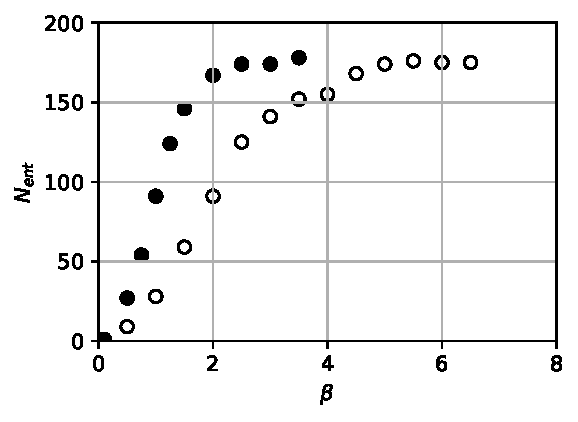
\includegraphics[width=\linewidth]{result-nanopore-eq-nent-by-beta-qfi-wyi}
	\caption{
		Нанопора заполненная спин-несущими частицами.
	}
	\label{fig:result-nanopore-eq-nent-by-beta-qfi-wyi}
  \end{subfigure}
  \hfill
  \begin{subfigure}[t]{0.49\textwidth}
    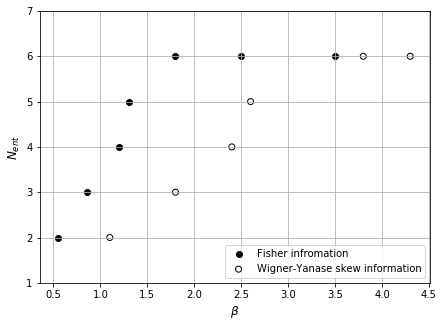
\includegraphics[width=\linewidth]{result-zchain-nent-by-beta-qfi-wyi}
	\caption{
		Зигзагообразная цепочка, состоящей из шести спинов.
	}
	\label{fig:result-zchain-nent-by-beta-qfi-wyi}
  \end{subfigure}
  \caption{
    Зависимость оценки снизу числа запутанных спинов  $N_\mathrm{ent}$
	от параметра обратной температуры $\beta = \frac{\pi \omega_0}{kT}$
	Черные круги --- результаты полученные на основе квантовой информации Фишера.
	Белые круги --- результаты полученные на основе косой информации Вигнера-Янасе.
  }
  \label{fig:result-nent-by-beta-qfi-wyi}
\end{figure}

Величины квантовой информации Фишера~$I_\mathrm{F}(\rho(\tau,\beta),I_z)$ и косой информации Вигнера-Яанасе~$I_{WY}(\rho(\tau,\beta),I_z)$
связаны с количеством запутанных частиц в системе (см. раздел~\ref{sec:manyparticle-entanglement-criteria}).
Если величина информации превышает значение $mk^2 + (N - mk)^2$,
где $k, m$ целые числа и $m$ --- это целая часть $N/k$,
тогда гарантируется,
что в системе как минимум $k+1$ частиц связаны в одно несепарабельное состояние.

В разделе~\ref{sec:qfi-wyi-comparison} было получено следующее неравенство
для квантовой информации Фишера и косой информации Вигнера-Янасе:
%
\begin{equation} \label{eq:qfi-wyi-inequality}
    I_{WY}\left(\rho(\tau,\beta), I_z\right)
    \leq I_F\left(\rho(\tau,\beta), I_z\right)
    \leq 2I_{WY}\left(\rho(\tau,\beta), I_z\right).
\end{equation}
%
Неравенство~(\ref{eq:qfi-wyi-inequality}) позволяет надеяться,
что полученные результаты для оценки числа запутанных спинов не будут значительно отличаться.

На Рис.~\ref{fig:result-nent-by-beta-qfi-wyi} представлены результаты зависимости
оценки снизу количества запутанных частиц в системе от обратной температуры $\beta$.
Оценки количества запутанных частиц были полученных на основе квантовой информации Фишера и косой информации Вигнера-Янасе.
Величины обеих информаций были вычислены через второй момент распределения МК когерентностей ЯМР~(cм.
разделы~\ref{sec:reduced-mq-coherences}~и~\ref{sec:wyi-mesuarement}).
На Рис.~\ref{fig:result-nanopore-eq-nent-by-beta-qfi-wyi} сравнение проведено для модели несферической нанопоры,
заполненной газом спин-несущих атомов (например, ксеноном) или молекул в сильном внешнем магнитном поле~(см. раздел~\ref{sec:model-equivalent-spins}).
Расчеты второго момента $M_2(\tau, \beta)$ были сделаны по аналогии с разделом~\ref{sec:nanopora-thermodynamic-equilibrium} для системы из 201 спина.
На Рис.~\ref{fig:result-zchain-nent-by-beta-qfi-wyi} сравнение проведено
для модели зигзагообразной цепочки ядерных спинов в кристалле гамбергита~(см. раздел~\ref{sec:model-zigzag-chain}).
Расчеты второго момента $M_2(\tau, \beta)$ были сделаны по аналогии с главой~\ref{chapter:manayparticle-entantlement-in-zigzag-chain}

% \section{Обобщения косой информации}
% \begin{align}
%     I_{WY}\left( \rho(t, T), I_z \right) & = 2\sum\limits_k k^2 J_k(t, 2T) = 2M_2(t, 2T) \\
%     I_{WYG}\left( \rho(t, T), I_z \right) &  = -2 \tr{\left[\rho(t, T), I_z\right]} = 2M_2(t, T) \\
%     I_{WYD} \left( \rho(t, T), I_z \right) &  = -2 \mathrm{Tr} \left\{
%         \left[\rho^\alpha, I_z \right] \left[\rho^{1 - \alpha}, I_z \right]
%     \right\}
% \end{align}

\section{Выводы}
Косая информация Вигнера-Янасе, так же как и информация Фишера,
является одной из важнейших мер в теории квантовой информации.
Полученный в этом разделе результат открывает множество возможностей
экспериментального исследования косой информации в различных системах.
В частности, она может быть применена для экспериментального исследования многочастичной запутанности.
Подобные исследования многочастичной запутанности требуют крайне низких температур $<10^{-3}$~K.
В этом случае информация Вигнера-Янасе имеет существенное преимущество перед информацией Фишера,
так как измерение первой для системы с температурой $T$
может быть проведено на установке с вдвое большей температурой $2T$.
